\documentclass[aspectratio=169,12pt]{beamer}

% =============================================================================
% THEME & COLORS
% =============================================================================
\usetheme{Madrid}
\usecolortheme{default}

\definecolor{mnit}{RGB}{0,51,102}
\definecolor{mnitlight}{RGB}{0,102,153}
\definecolor{mnitaccent}{RGB}{204,85,0}

\setbeamercolor{palette primary}{bg=mnit,fg=white}
\setbeamercolor{palette secondary}{bg=mnitlight,fg=white}
\setbeamercolor{palette tertiary}{bg=mnit,fg=white}
\setbeamercolor{structure}{fg=mnit}
\setbeamercolor{title}{fg=white,bg=mnit}
\setbeamercolor{frametitle}{fg=white,bg=mnit}
\setbeamercolor{block title}{bg=mnit,fg=white}
\setbeamercolor{block body}{bg=mnit!10,fg=black}
\setbeamercolor{item}{fg=mnit}

\setbeamertemplate{navigation symbols}{}
\setbeamertemplate{footline}{}

% =============================================================================
% PACKAGES
% =============================================================================
\usepackage{graphicx}
\usepackage{booktabs}
\usepackage{amsmath}
\usepackage{array}
\usepackage{multicol}
\usepackage{tikz}
\usepackage{listings}
\usepackage{xcolor}

\lstset{
    basicstyle=\ttfamily\tiny,
    breaklines=true,
    frame=single,
    backgroundcolor=\color{gray!10}
}

% =============================================================================
% TITLE INFO
% =============================================================================
\title[Hybrid Phishing Detection]{Intelligent Hybrid Phishing Detection using\\URL Analysis, Vision Models, and LLM Reasoning}
\author[Dhruv \& Govind]{Dhruv Khandelwal (2022UCP1130)\\Govind Ram Mali (2022UCP1630)}
\institute[MNIT Jaipur]{
    Department of Computer Science \& Engineering\\
    Malaviya National Institute of Technology Jaipur\\[0.3cm]
    \textbf{Supervisor:} Dr.\ Arka Prokash Mazumdar
}
\date{May 2026}
\titlegraphic{\includegraphics[height=1.2cm]{Mnit_logo.png}}

\begin{document}

% ======================= SLIDE 1: TITLE =======================
\begin{frame}[plain]
    \titlepage
\end{frame}

% ======================= SLIDE 2: OUTLINE =======================
\begin{frame}{Outline}
    \tableofcontents
\end{frame}

% ======================= SECTION: INTRODUCTION =======================
\section{Introduction}

% ======================= SLIDE 3: INTRODUCTION =======================
\begin{frame}{Introduction}
    \begin{itemize}
        \item \textbf{Phishing} --- fraudulent websites mimicking legitimate ones to steal sensitive information (credentials, financial data, personal details)
        \vspace{0.3cm}
        \item Phishing attacks increased by \textbf{over 60\%} in the past year, with millions of phishing sites detected monthly
        \vspace{0.3cm}
        \item Traditional single-modality detection systems face critical limitations:
        \begin{itemize}
            \item URL-based methods evaded via obfuscation, typosquatting, homograph attacks
            \item Content-based methods fail against sophisticated visual mimicry
            \item Lack of \textbf{interpretability} in detection decisions
        \end{itemize}
        \vspace{0.3cm}
        \item \textbf{Need:} A multi-modal, interpretable, and real-time detection system
    \end{itemize}
\end{frame}

% ======================= SECTION: PROBLEM STATEMENT =======================
\section{Problem Statement}

% ======================= SLIDE 4: PROBLEM STATEMENT =======================
\begin{frame}{Problem Statement}
    \begin{block}{Core Challenge}
        Design a \textbf{robust, accurate, and interpretable} phishing detection system overcoming limitations of single-modality approaches.
    \end{block}
    \vspace{0.4cm}
    The system must:
    \begin{enumerate}
        \item Analyze \textbf{multiple characteristics} --- URL structure, visual appearance, semantic content
        \item Provide \textbf{real-time detection} with sub-second latency
        \item Generate \textbf{human-readable explanations} for decisions
        \item Achieve \textbf{high accuracy} with low false positive rates
        \item \textbf{Adapt} to evolving phishing techniques via modern ML/DL architectures
    \end{enumerate}
\end{frame}

% ======================= SECTION: LITERATURE REVIEW =======================
\section{Literature Review}

% ======================= SLIDE 5: LITERATURE REVIEW =======================
\begin{frame}{Literature Review}
    \footnotesize
    \begin{table}
        \centering
        \begin{tabular}{p{2cm}p{4.2cm}p{4.2cm}}
            \toprule
            \textbf{Approach} & \textbf{Key Work} & \textbf{Limitations} \\
            \midrule
            URL-Based & Ma et al.\ (2009), URLNet (2018) & Cannot detect visual mimicry; susceptible to obfuscation \\
            Visual-Based & GoldPhish (2010), PhishPedia (2021) & Misses URL indicators; computationally expensive \\
            Content-Based & CANTINA (2007), DeltaPhish (2017) & Requires page access; evaded by dynamic content \\
            Blacklist & PhishNet (2010) & Cannot detect zero-day attacks \\
            Multi-Modal & Marchal et al.\ (2017) & Lacks interpretability; no LLM integration \\
            \bottomrule
        \end{tabular}
    \end{table}
    \vspace{0.2cm}
    \begin{alertblock}{Research Gap}
        No existing system combines URL + Visual + LLM explainability in a unified framework.
    \end{alertblock}
\end{frame}

% ======================= SECTION: OBJECTIVES =======================
\section{Objectives}

% ======================= SLIDE 6: OBJECTIVES =======================
\begin{frame}{Objectives}
    \begin{enumerate}
        \item \textbf{Multi-Modal Analysis} --- Combine URL features, visual screenshots, and semantic understanding
        \vspace{0.2cm}
        \item \textbf{ML Pipeline} --- Train XGBoost, Random Forest, LightGBM on 30+ URL features
        \vspace{0.2cm}
        \item \textbf{Deep Learning Integration} --- ResNet, Vision Transformer, EfficientNet for visual analysis
        \vspace{0.2cm}
        \item \textbf{Explainable AI} --- LLM-generated human-readable explanations (GPT-4 / HuggingFace)
        \vspace{0.2cm}
        \item \textbf{Fusion Strategies} --- Weighted averaging, voting, stacking for combining modalities
        \vspace{0.2cm}
        \item \textbf{Production-Ready} --- REST API, batch processing, and web frontend
    \end{enumerate}
\end{frame}

% ======================= SECTION: PROPOSED METHODOLOGY =======================
\section{Proposed Methodology}

% ======================= SLIDE 7: SYSTEM ARCHITECTURE =======================
\begin{frame}{System Architecture}
    \begin{figure}
        \centering
        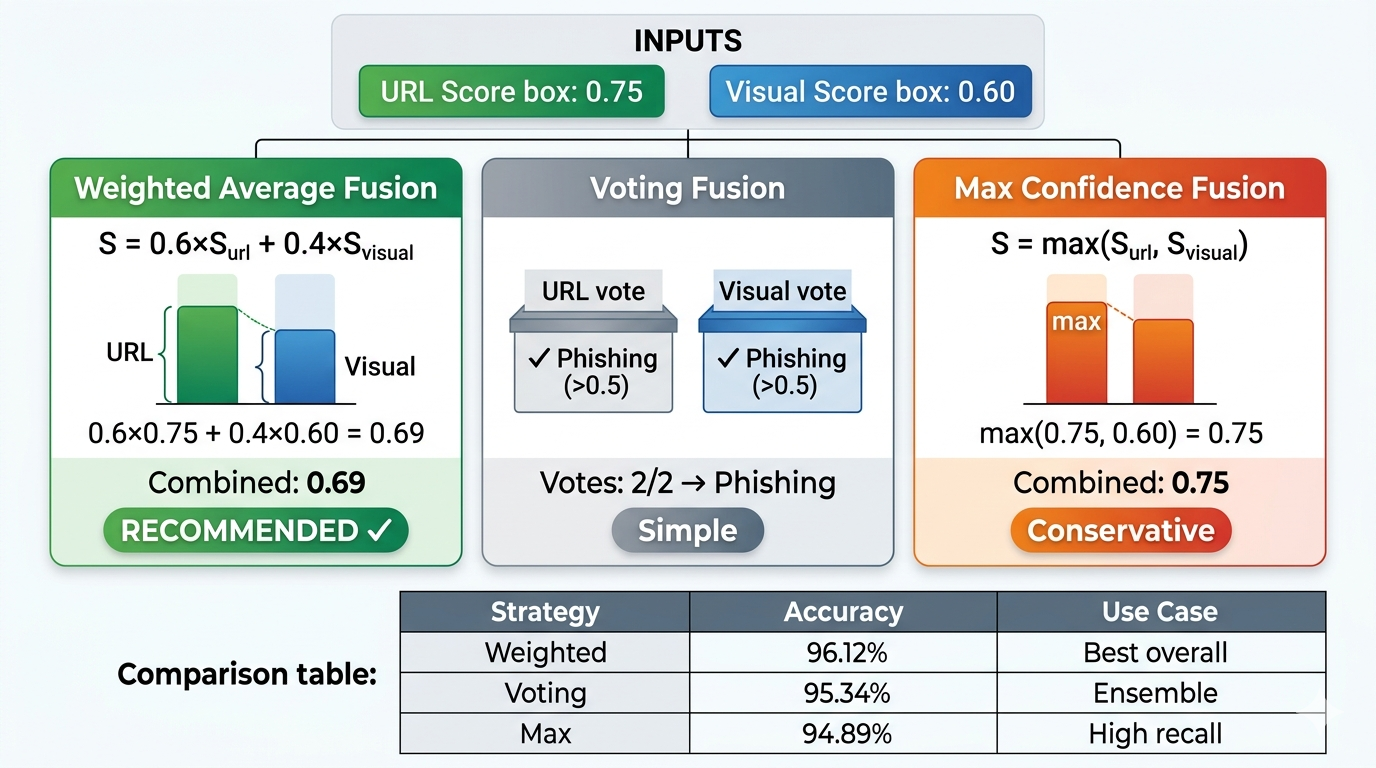
\includegraphics[width=0.78\textwidth]{system_architecture.png}
        \caption{Hybrid Multi-Modal Phishing Detection Architecture}
    \end{figure}
\end{frame}

% ======================= SLIDE 9: URL ANALYSIS MODULE =======================
\begin{frame}{URL Analysis Module}
    \begin{columns}[T]
        \begin{column}{0.48\textwidth}
            \textbf{30+ Extracted Features:}
            \begin{itemize}
                \small
                \item \textbf{Structural:} URL length, domain length, path length, subdomain count
                \item \textbf{Character:} Dots, hyphens, digit ratio, special chars
                \item \textbf{Security:} HTTPS, IP address, port, @ symbol
                \item \textbf{Lexical:} Shannon entropy, sensitive words, suspicious TLD
                \item \textbf{Patterns:} Redirects, hex encoding, punycode
            \end{itemize}
        \end{column}
        \begin{column}{0.48\textwidth}
            \textbf{Shannon Entropy:}
            \[
            H(URL) = -\sum_{i=1}^{n} p(c_i) \log_2 p(c_i)
            \]
            \vspace{0.3cm}
            \textbf{ML Models:}
            \begin{itemize}
                \small
                \item XGBoost (best performer)
                \item Random Forest
                \item LightGBM
            \end{itemize}
        \end{column}
    \end{columns}
    \vspace{0.3cm}
    \begin{figure}
        \centering
        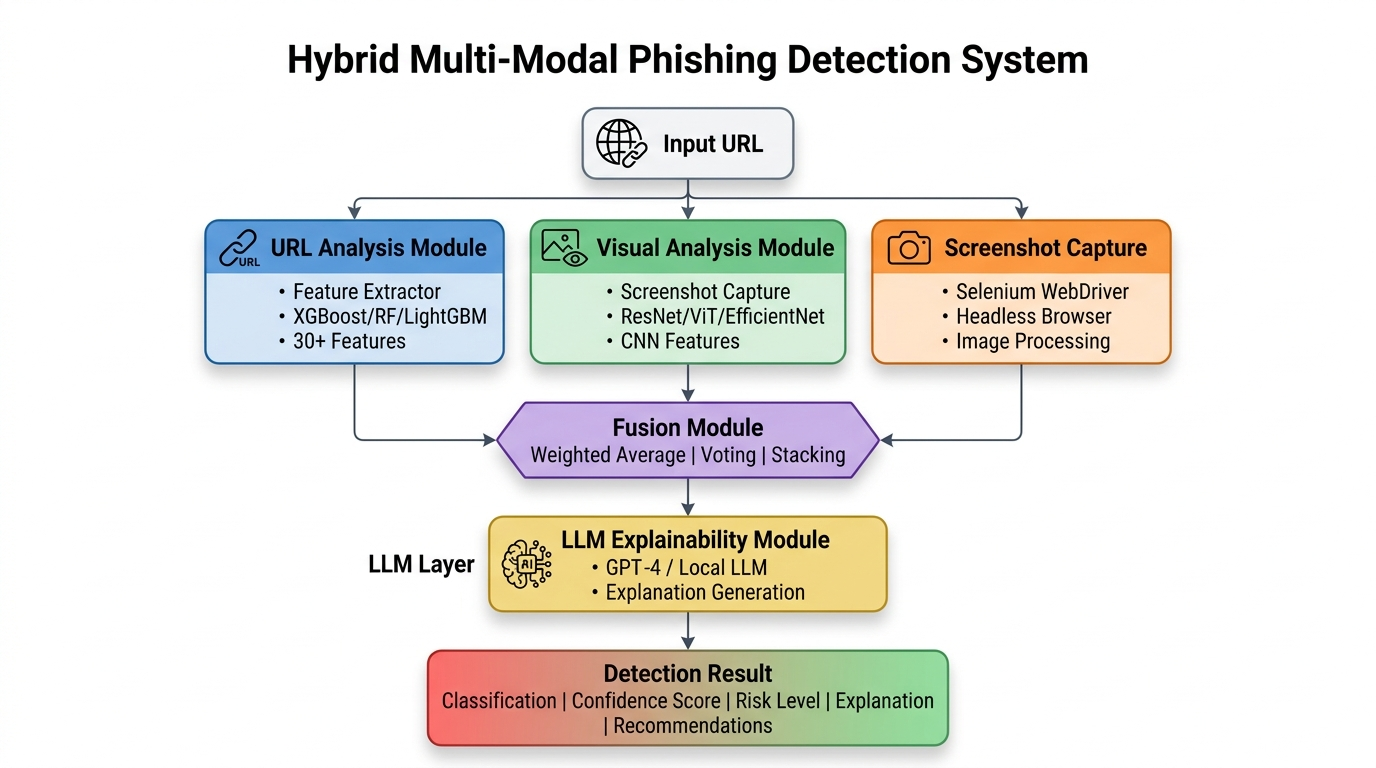
\includegraphics[width=0.55\textwidth]{ml_ensemble.png.png}
    \end{figure}
\end{frame}

% ======================= SLIDE 10: VISUAL ANALYSIS MODULE =======================
\begin{frame}{Visual Analysis Module}
    \begin{columns}[T]
        \begin{column}{0.45\textwidth}
            \textbf{Architectures:}
            \begin{itemize}
                \item \textbf{ResNet-50/101} --- Skip connections for deep networks
                \item \textbf{Vision Transformer (ViT)} --- Global dependencies via attention
                \item \textbf{EfficientNet} --- Compound scaling
            \end{itemize}
            \vspace{0.3cm}
            \textbf{Preprocessing:}
            \begin{itemize}
                \small
                \item Resize to $224 \times 224$
                \item ImageNet normalization
                \item Augmentation: crops, flips, color jitter
            \end{itemize}
        \end{column}
        \begin{column}{0.52\textwidth}
            \begin{figure}
                \centering
                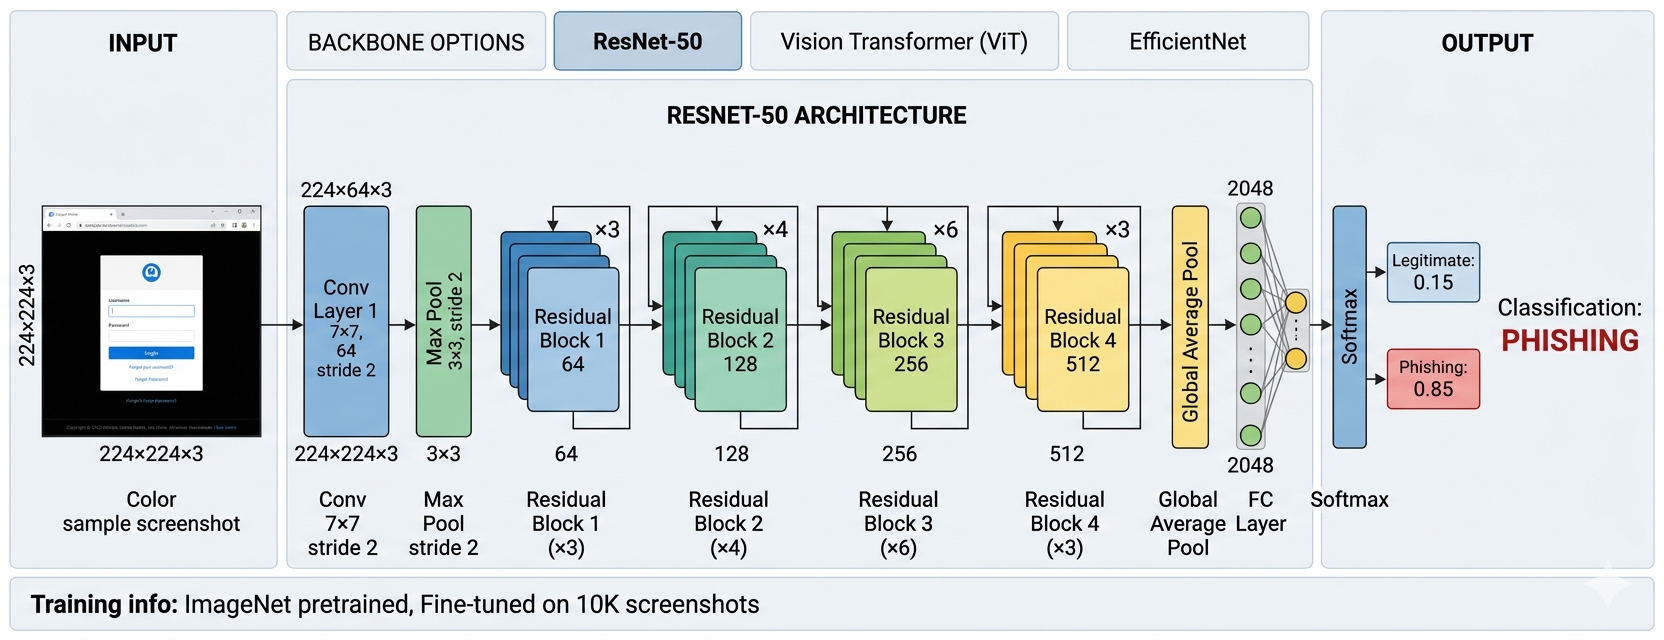
\includegraphics[width=\textwidth]{visual_model_architecture.png}
            \end{figure}
        \end{column}
    \end{columns}
\end{frame}

% ======================= SLIDE 11b: LLM EXPLAINABILITY =======================
\begin{frame}{LLM Explainability Module}
    \begin{columns}[T]
        \begin{column}{0.48\textwidth}
            \textbf{LLM Integration:}
            \begin{itemize}
                \item GPT-4 / HuggingFace local models
                \item Receives URL + scores + detected indicators
                \item Generates human-readable output
                \item Improves user trust \& transparency
            \end{itemize}
        \end{column}
        \begin{column}{0.48\textwidth}
            \textbf{Output for each URL:}
            \begin{enumerate}
                \item Classification result
                \item Confidence score (0--1)
                \item Detailed explanation
                \item Risk assessment
                \item Security recommendations
            \end{enumerate}
        \end{column}
    \end{columns}
\end{frame}

% ======================= SLIDE 11c: FUSION STRATEGIES =======================
\begin{frame}{Fusion Strategies}
    \begin{figure}
        \centering
        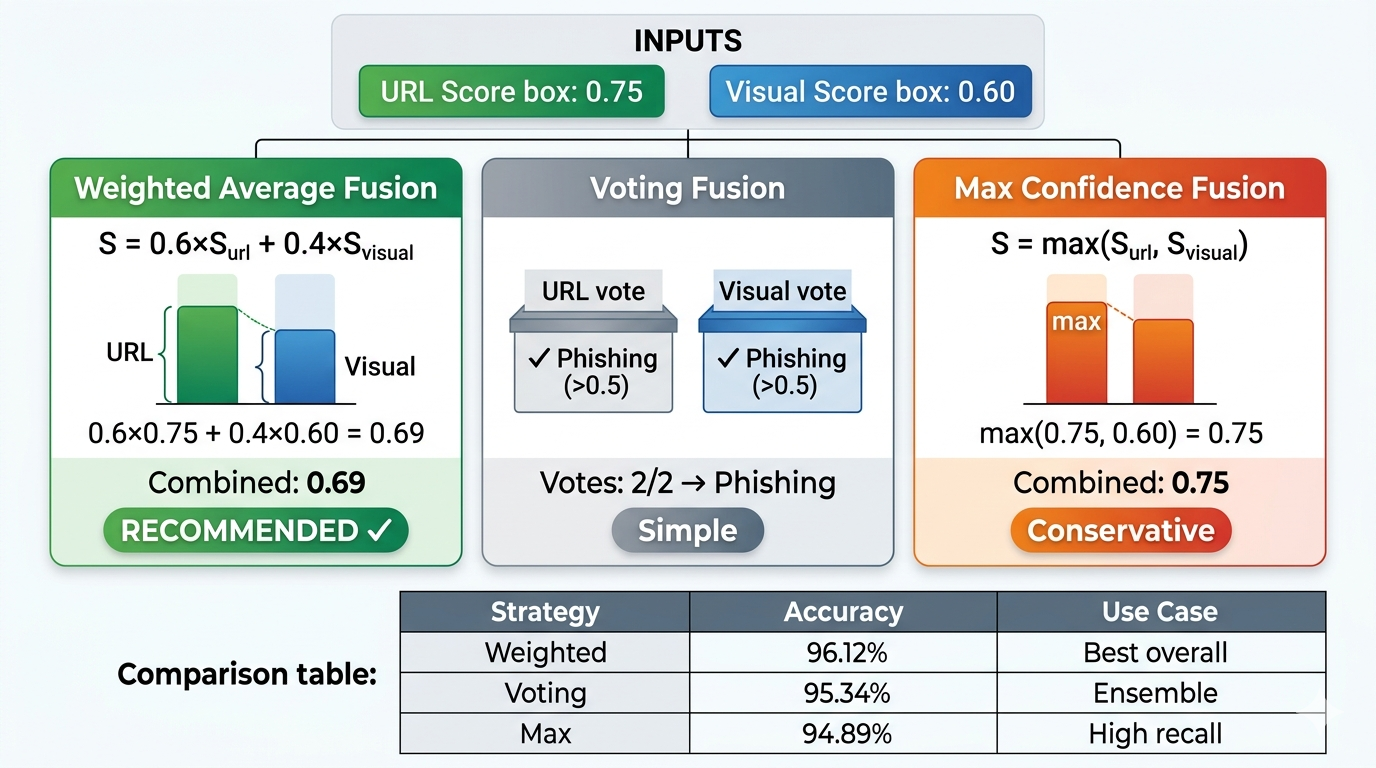
\includegraphics[width=0.78\textwidth]{fusion_strategies.png}
        \caption{Comparison of Multi-Modal Fusion Strategies}
    \end{figure}
\end{frame}

% ======================= SECTION: EXPERIMENTAL SETUP =======================
\section{Experimental Setup}

% ======================= SLIDE 12: EXPERIMENTAL SETUP =======================
\begin{frame}{Experimental Setup}
    \begin{columns}[T]
        \begin{column}{0.48\textwidth}
            \textbf{Datasets:}
            \begin{itemize}
                \item Synthetic --- 2000 URLs (50/50 split)
                \item PhishTank --- Real phishing URLs
                \item Alexa Top Sites --- Legitimate URLs
                \item Screenshot Dataset --- Visual training data
            \end{itemize}
            \vspace{0.3cm}
            \textbf{Evaluation Metrics:}
            \begin{itemize}
                \item Accuracy, Precision, Recall
                \item F1-Score, ROC-AUC
                \item Inference Time
            \end{itemize}
        \end{column}
        \begin{column}{0.48\textwidth}
            \textbf{Technology Stack:}
            \small
            \begin{tabular}{ll}
                \toprule
                \textbf{Component} & \textbf{Tool} \\
                \midrule
                Language & Python 3.9+ \\
                ML & scikit-learn, XGBoost \\
                DL & PyTorch 2.0+, timm \\
                API & FastAPI \\
                Screenshot & Selenium \\
                LLM & OpenAI, HuggingFace \\
                Testing & pytest \\
                \bottomrule
            \end{tabular}
        \end{column}
    \end{columns}
\end{frame}

% ======================= SECTION: RESULTS =======================
\section{Results and Analysis}

% ======================= SLIDE 13: URL MODEL RESULTS =======================
\begin{frame}{URL Model Results}
    \begin{table}
        \centering
        \small
        \begin{tabular}{lccccc}
            \toprule
            \textbf{Model} & \textbf{Accuracy} & \textbf{Precision} & \textbf{Recall} & \textbf{F1} & \textbf{AUC} \\
            \midrule
            \textbf{XGBoost} & \textbf{0.9456} & \textbf{0.9423} & \textbf{0.9512} & \textbf{0.9467} & \textbf{0.9821} \\
            Random Forest & 0.9387 & 0.9356 & 0.9445 & 0.9400 & 0.9756 \\
            LightGBM & 0.9412 & 0.9389 & 0.9478 & 0.9433 & 0.9789 \\
            \bottomrule
        \end{tabular}
        \caption{URL Model Performance Comparison}
    \end{table}
    \vspace{0.2cm}
    \textbf{Top Features:} \texttt{num\_sensitive\_words} (0.152), \texttt{entropy} (0.129), \texttt{url\_length} (0.095), \texttt{has\_https} (0.082), \texttt{num\_subdomains} (0.076)
\end{frame}

% ======================= SLIDE 14: VISUAL MODEL RESULTS =======================
\begin{frame}{Visual Model Results}
    \begin{table}
        \centering
        \small
        \begin{tabular}{lcccc}
            \toprule
            \textbf{Architecture} & \textbf{Accuracy} & \textbf{F1-Score} & \textbf{ROC-AUC} & \textbf{Inference} \\
            \midrule
            ResNet-50 & 0.9234 & 0.9201 & 0.9678 & 45ms \\
            ResNet-101 & 0.9312 & 0.9278 & 0.9723 & 68ms \\
            \textbf{ViT-Base} & \textbf{0.9389} & \textbf{0.9356} & \textbf{0.9789} & 52ms \\
            EfficientNet-B0 & 0.9178 & 0.9145 & 0.9634 & 32ms \\
            \bottomrule
        \end{tabular}
        \caption{Visual Model Performance Comparison}
    \end{table}
    \vspace{0.3cm}
    \begin{itemize}
        \item Vision Transformer (ViT) achieves the \textbf{best accuracy and AUC}
        \item EfficientNet offers the \textbf{fastest inference} (32ms)
        \item All architectures use \textbf{ImageNet pretrained} weights with fine-tuning
    \end{itemize}
\end{frame}

% ======================= SLIDE 15: HYBRID SYSTEM RESULTS =======================
\begin{frame}{Hybrid System Results}
    \begin{columns}[T]
        \begin{column}{0.52\textwidth}
            \begin{table}
                \centering
                \tiny
                \begin{tabular}{lcccc}
                    \toprule
                    \textbf{System} & \textbf{Acc} & \textbf{Prec} & \textbf{Rec} & \textbf{F1} \\
                    \midrule
                    URL Only & .9456 & .9423 & .9512 & .9467 \\
                    Visual Only & .9234 & .9189 & .9312 & .9250 \\
                    \textbf{Hybrid (Wt.\ Avg)} & \textbf{.9612} & \textbf{.9578} & \textbf{.9656} & \textbf{.9617} \\
                    Hybrid (Voting) & .9534 & .9501 & .9589 & .9545 \\
                    Hybrid (Max) & .9489 & .9456 & .9534 & .9495 \\
                    \bottomrule
                \end{tabular}
            \end{table}
            \vspace{0.2cm}
            \begin{alertblock}{Key Finding}
                Hybrid weighted average achieves \textbf{96.12\% accuracy}, surpassing URL-only by \textbf{+1.56\%} and visual-only by \textbf{+3.78\%}.
            \end{alertblock}
        \end{column}
        \begin{column}{0.45\textwidth}
            \begin{figure}
                \centering
                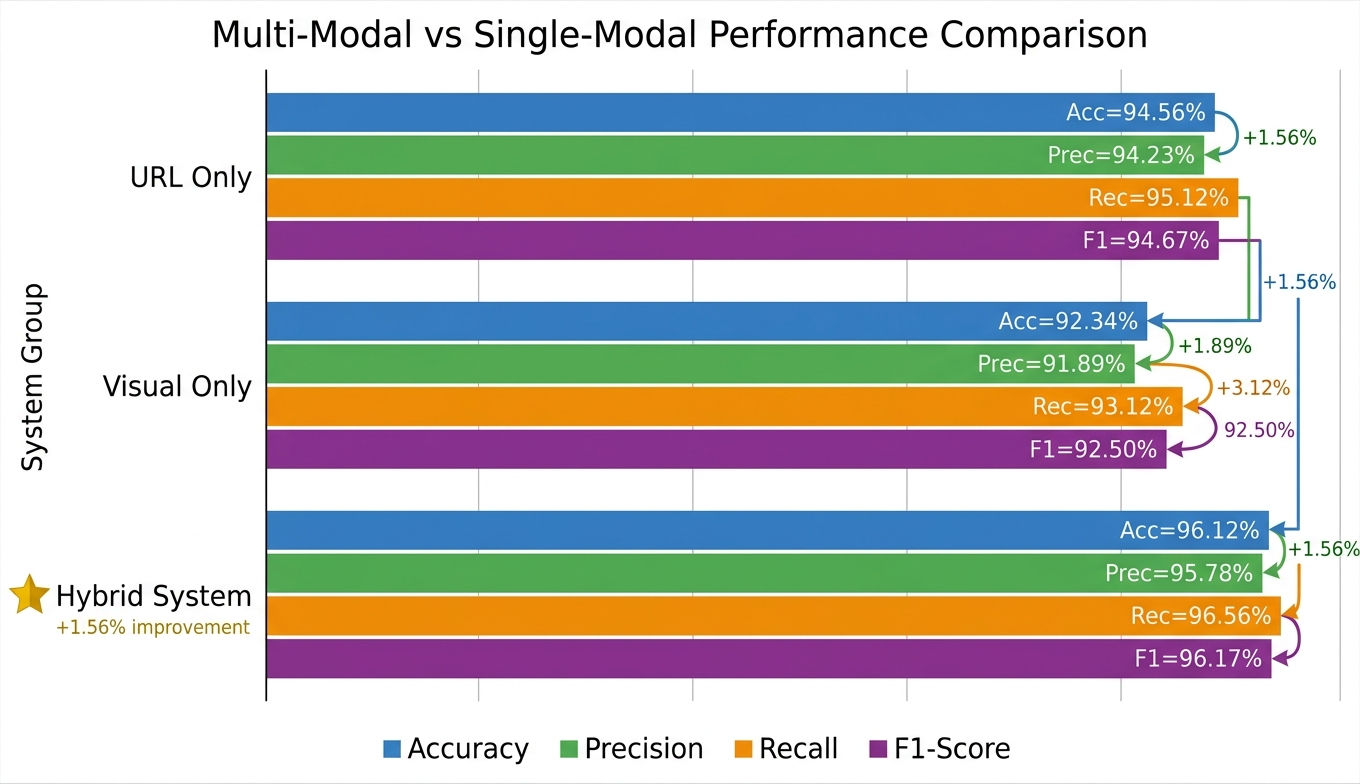
\includegraphics[width=\textwidth]{performance_comparison.png}
                \caption{Performance Comparison}
            \end{figure}
        \end{column}
    \end{columns}
\end{frame}

% ======================= SLIDE 16: PERFORMANCE STATS =======================
\begin{frame}{System Performance}
    \begin{table}
        \centering
        \begin{tabular}{lc}
            \toprule
            \textbf{Metric} & \textbf{Value} \\
            \midrule
            Avg.\ Analysis Time (URL only) & 12ms \\
            Avg.\ Analysis Time (with screenshot) & 850ms \\
            Avg.\ Analysis Time (full + LLM) & 1.2s \\
            Throughput (URL only) & 83 URLs/sec \\
            Memory Usage (loaded models) & 512MB \\
            API Response (95th percentile) & 150ms \\
            \bottomrule
        \end{tabular}
        \caption{Runtime Performance Metrics}
    \end{table}
    \vspace{0.3cm}
    \begin{block}{Threshold Analysis}
        Optimal threshold $= 0.5$ yields the best F1-score (0.9467), balancing precision (0.9423) and recall (0.9512).
    \end{block}
\end{frame}

% ======================= SECTION: CONCLUSION =======================
\section{Conclusion and Future Scope}

% ======================= SLIDE 17: CONCLUSION =======================
\begin{frame}{Conclusion}
    \textbf{Key Contributions:}
    \begin{enumerate}
        \item \textbf{Multi-Modal Architecture} --- URL + Visual + LLM for comprehensive detection
        \item \textbf{Explainable Detection} --- LLM-generated human-readable explanations
        \item \textbf{Flexible Fusion} --- Weighted average, voting, max confidence strategies
        \item \textbf{Production-Ready} --- REST API, batch processing, web interface
    \end{enumerate}
    \vspace{0.4cm}
    \textbf{Key Findings:}
    \begin{itemize}
        \item Hybrid system: \textbf{96.12\%} accuracy (vs.\ 94.56\% URL-only, 92.34\% visual-only)
        \item XGBoost --- best URL model; ViT --- best visual model
        \item Weighted average fusion outperforms other strategies
        \item LLM explanations improve user trust and understanding
    \end{itemize}
\end{frame}

% ======================= SLIDE 18: FUTURE SCOPE =======================
\begin{frame}{Future Scope}
    \begin{columns}[T]
        \begin{column}{0.48\textwidth}
            \begin{itemize}
                \item \textbf{Real-Time Streaming} --- Continuous URL stream monitoring
                \vspace{0.3cm}
                \item \textbf{Adversarial Robustness} --- Defenses against evasion attacks
                \vspace{0.3cm}
                \item \textbf{Brand-Specific Models} --- Specialized detection for banking, social media
                \vspace{0.3cm}
                \item \textbf{Mobile Deployment} --- Lightweight models for mobile devices
            \end{itemize}
        \end{column}
        \begin{column}{0.48\textwidth}
            \begin{itemize}
                \item \textbf{Federated Learning} --- Privacy-preserving collaborative training
                \vspace{0.3cm}
                \item \textbf{Multilingual Support} --- Detection across languages and scripts
                \vspace{0.3cm}
                \item \textbf{Zero-Shot Detection} --- Detecting phishing for unseen brands
                \vspace{0.3cm}
                \item \textbf{Browser Extension} --- Real-time user protection
            \end{itemize}
        \end{column}
    \end{columns}
\end{frame}

% ======================= SLIDE 19: PROJECT DEMO 1 =======================
\begin{frame}{Project Demo --- Page 1}
    \vspace{-0.3cm}
    \begin{columns}[c]
        \begin{column}{0.5\textwidth}
            \begin{figure}
                \centering
                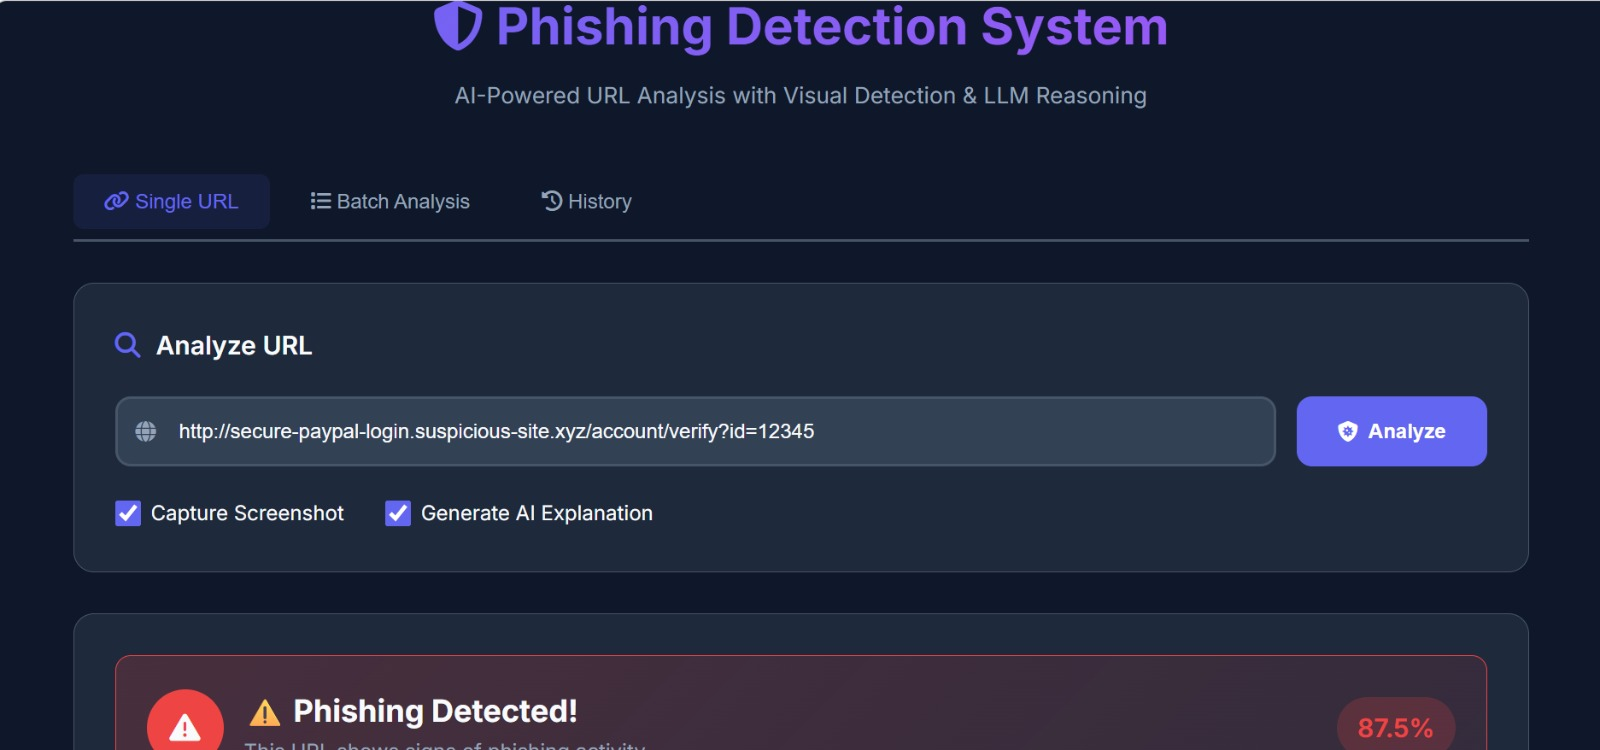
\includegraphics[width=\textwidth,height=\textheight,keepaspectratio]{ps1.jpeg}
            \end{figure}
        \end{column}
        \begin{column}{0.5\textwidth}
            \begin{figure}
                \centering
                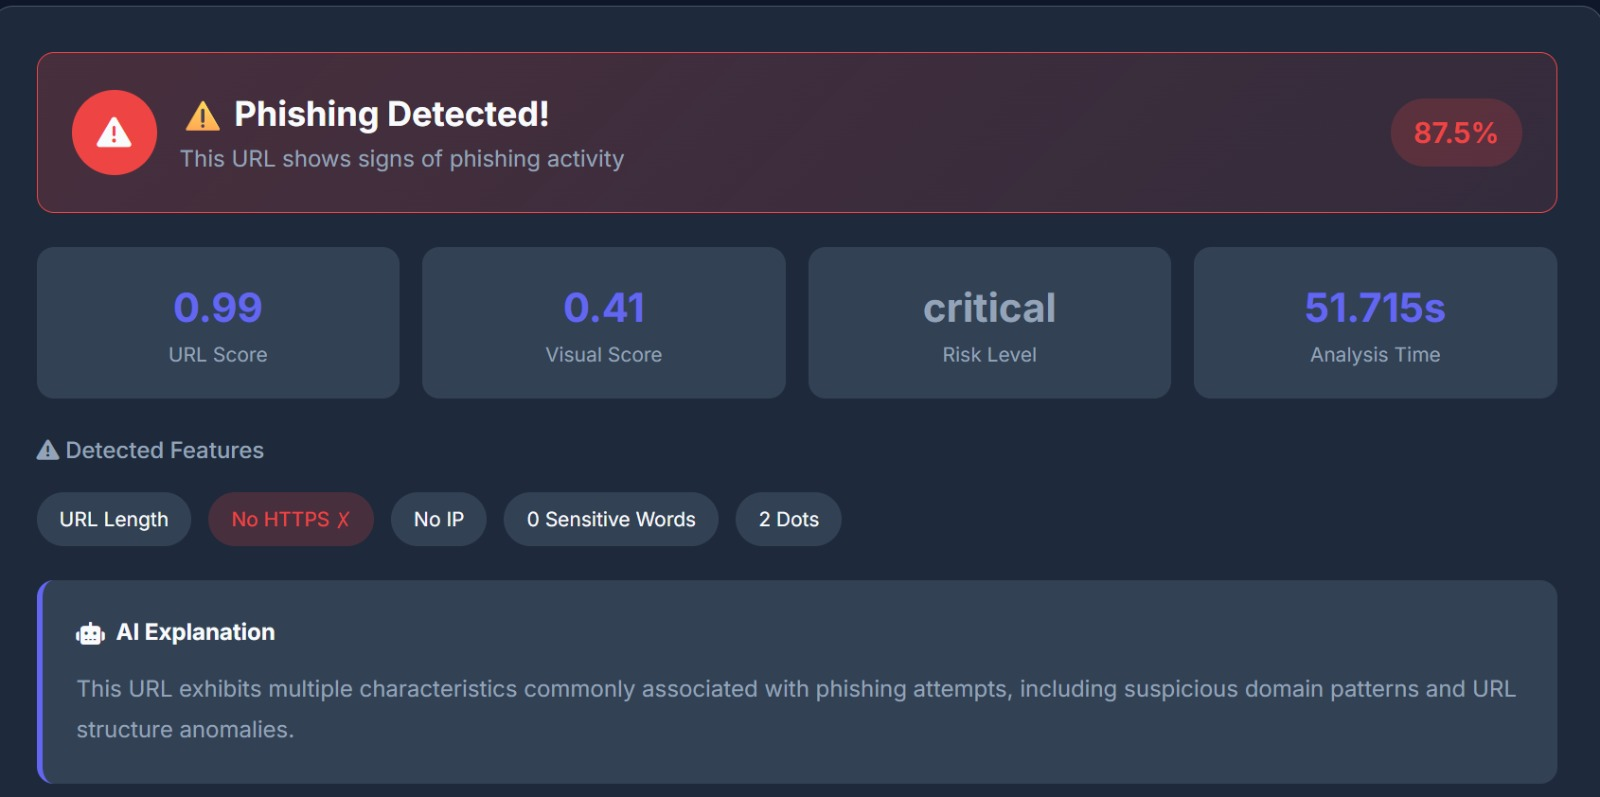
\includegraphics[width=\textwidth,height=\textheight,keepaspectratio]{ps2.jpeg}
            \end{figure}
        \end{column}
    \end{columns}
\end{frame}

% ======================= SLIDE 20: PROJECT DEMO 2 =======================
\begin{frame}{Project Demo --- Page 2}
    \vspace{-0.3cm}
    \begin{columns}[c]
        \begin{column}{0.5\textwidth}
            \begin{figure}
                \centering
                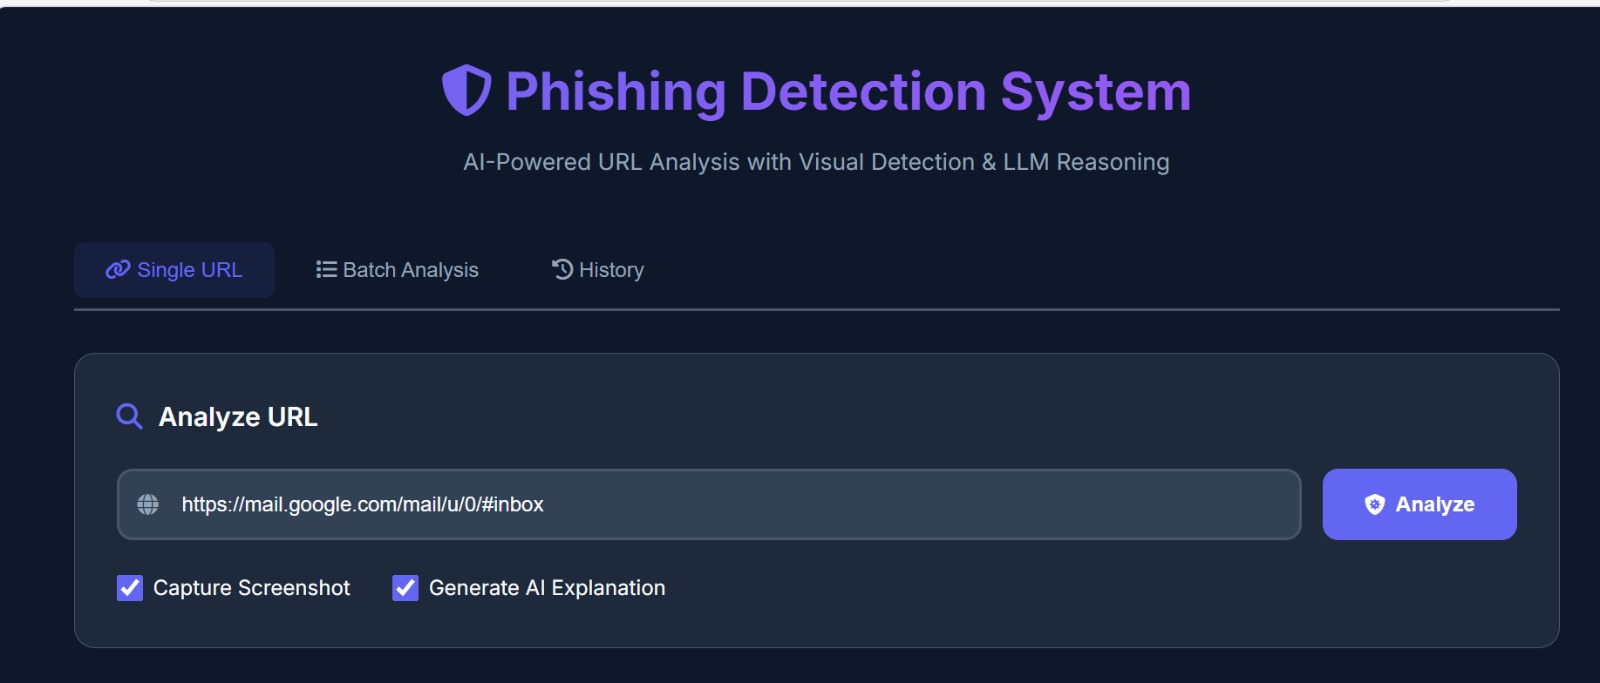
\includegraphics[width=\textwidth,height=\textheight,keepaspectratio]{sf1.jpeg}
            \end{figure}
        \end{column}
        \begin{column}{0.5\textwidth}
            \begin{figure}
                \centering
                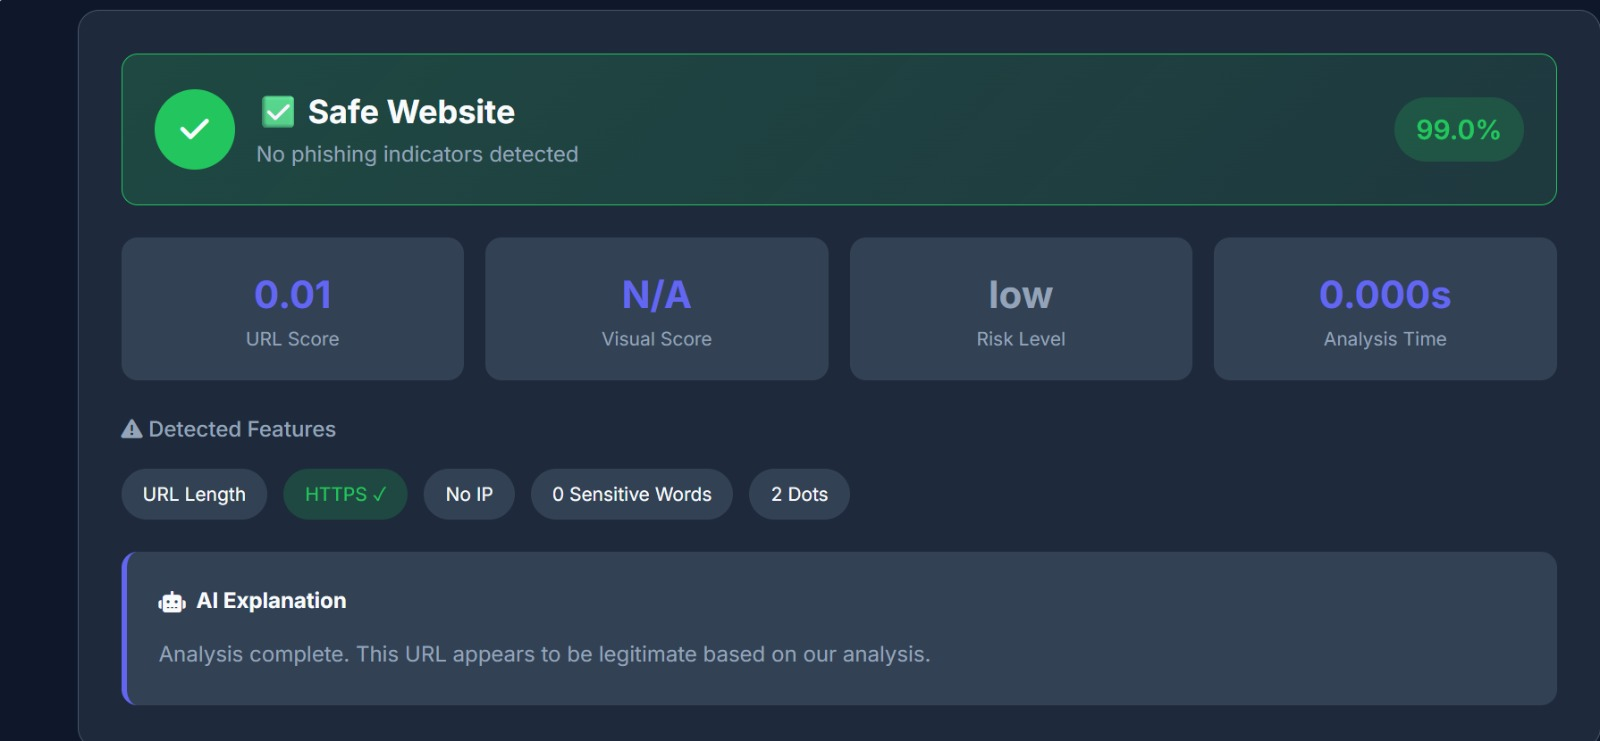
\includegraphics[width=\textwidth,height=\textheight,keepaspectratio]{sf2.jpeg}
            \end{figure}
        \end{column}
    \end{columns}
\end{frame}

% ======================= SECTION: REFERENCES =======================
\section{References}

% ======================= SLIDE 19: REFERENCES =======================
\begin{frame}[allowframebreaks]{References}
    \tiny
    \begin{thebibliography}{20}
        \bibitem{ma2009} J.\ Ma et al., ``Beyond blacklists: learning to detect malicious web sites from suspicious URLs,'' \textit{ACM SIGKDD}, 2009.
        \bibitem{mcgrath2008} D.K.\ McGrath and M.\ Gupta, ``Behind phishing: An examination of phisher modi operandi,'' \textit{USENIX LEET}, 2008.
        \bibitem{le2018} H.\ Le et al., ``URLNet: Learning a URL representation with deep learning for malicious URL detection,'' \textit{arXiv:1802.03162}, 2018.
        \bibitem{dunlop2010} M.\ Dunlop et al., ``GoldPhish: Using images for content-based phishing analysis,'' \textit{ICIMP}, 2010.
        \bibitem{lin2021} Y.\ Lin et al., ``Phishpedia: A Hybrid Deep Learning Based Approach to Visually Identify Phishing Webpages,'' \textit{USENIX Security}, 2021.
        \bibitem{marchal2017} S.\ Marchal et al., ``Off-the-hook: An efficient and usable client-side phishing prevention application,'' \textit{IEEE TC}, 2017.
        \bibitem{warnecke2020} A.\ Warnecke et al., ``Evaluating explanation methods for deep learning in security,'' \textit{IEEE EuroS\&P}, 2020.
        \bibitem{he2016} K.\ He et al., ``Deep residual learning for image recognition,'' \textit{IEEE CVPR}, 2016.
        \bibitem{dosovitskiy2020} A.\ Dosovitskiy et al., ``An image is worth 16x16 words: Transformers for image recognition at scale,'' \textit{arXiv:2010.11929}, 2020.
        \bibitem{chen2016} T.\ Chen and C.\ Guestrin, ``XGBoost: A scalable tree boosting system,'' \textit{ACM SIGKDD}, 2016.
        \bibitem{brown2020} T.\ Brown et al., ``Language models are few-shot learners,'' \textit{NeurIPS}, 2020.
        \bibitem{mohammad2014} R.M.\ Mohammad et al., ``Intelligent rule-based phishing websites classification,'' \textit{IET Inf.\ Sec.}, 2014.
        \bibitem{sahingoz2019} O.K.\ Sahingoz et al., ``Machine learning based phishing detection from URLs,'' \textit{Expert Syst.\ Appl.}, 2019.
    \end{thebibliography}
\end{frame}

% ======================= SLIDE 20: THANK YOU =======================
\begin{frame}[plain]
    \begin{center}
        \vspace{2cm}
        {\Huge\bfseries\color{mnit} Thank You!}
        \vspace{1cm}
        
        {\Large Questions?}
        \vspace{1.5cm}
        
        {\normalsize
        Dhruv Khandelwal (2022UCP1130)\\
        Govind Ram Mali (2022UCP1630)\\[0.5cm]
        Department of Computer Science \& Engineering\\
        MNIT Jaipur}
    \end{center}
\end{frame}

\end{document}
